\documentclass[12pt,a5paper]{article}

\usepackage[utf8]{inputenc}
\usepackage{geometry}
\usepackage{graphicx}
%\usepackage{hyperref}

\begin{document}

\tableofcontents
\listoffigures

\newpage
\section{Intorduction}

This game is a simple checkers (draughts) implementation, created as an university project. You may use it under MIT license.

In order to start game type “python3 main.py” while in the game folder.

\newpage
\section{Gameplay}

\subsection{Basics}
All pieces can move on a single diagonal in one move (exception: multiple captures).

In checkers there are basically two types of moves:
\begin{itemize}
	\item normal
	\item capture
\end{itemize}

When you want to perform a normal move you can change position of one of your pieces one step forward on a diagonal line (see figure~\ref{fig:first_move} on page~\pageref{fig:first_move}).
If you can perform a capture you are forced to do so.

Capture can be performed if the following circumstances are met:
\begin{itemize}
	\item it's your move
	\item one of your pieces “touches“ an opponent piece
	\item the field after the opponent piece on the diagonal is free
\end{itemize}
If, after a single capture, another capture could be performed the player is obligated to do so (see figure~\ref{fig:multiple_capture} on page~\pageref{fig:multiple_capture}).

\subsection{Kings}
After a player man reaches the last row, it becomes a king. Kings are allowed to move backwards and are not limited to move 1 or 2 fields depending on the situation (see figure~\ref{fig:capture_with_king} on page~\pageref{fig:capture_with_king}).

\subsection{Implemented rules}
The rules implemented in this version of checkcers are based on Russian draughts game variant. All implemented rules are listed bellow: 
\begin{itemize}
	\item multiple captures
	\item backward captures
	\item forced captures
	\item flaying kings
\end{itemize}

\newpage
\section{Usage}

After starting the game you should see screen looking like in the figure \ref{fig:start}.

\begin{figure}[h]
	\centering
	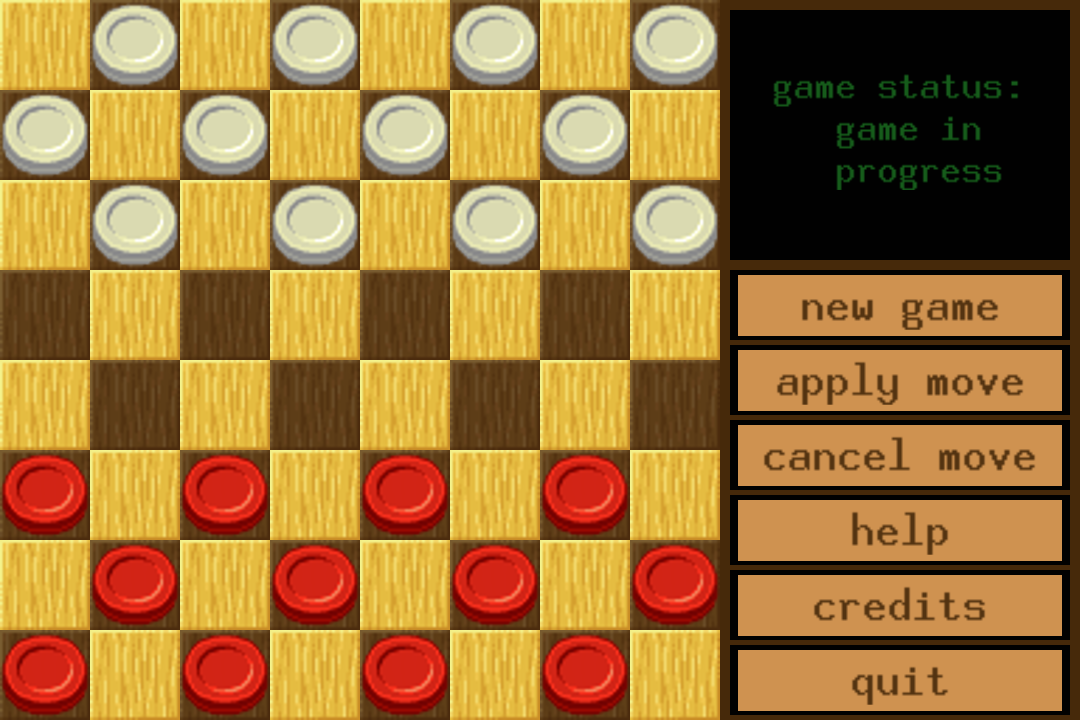
\includegraphics[width=8cm]{img/starting_position.png}
	\caption{Starting position}
	\label{fig:start}
\end{figure}

When you click on the board a number should appear. In order to move one of your pieces you have to select it with “1”. Then you have to point to every position your piece stops at. To see example of regular movement see figure~\ref{fig:first_move}, for capture figure~\ref{fig:capture} and \ref{fig:multiple_capture} for a multiple capture.\\
Kings can capture in the same way as is to see in figure~\ref{fig:capture_with_king}

\begin{figure}[h]
	\centering
	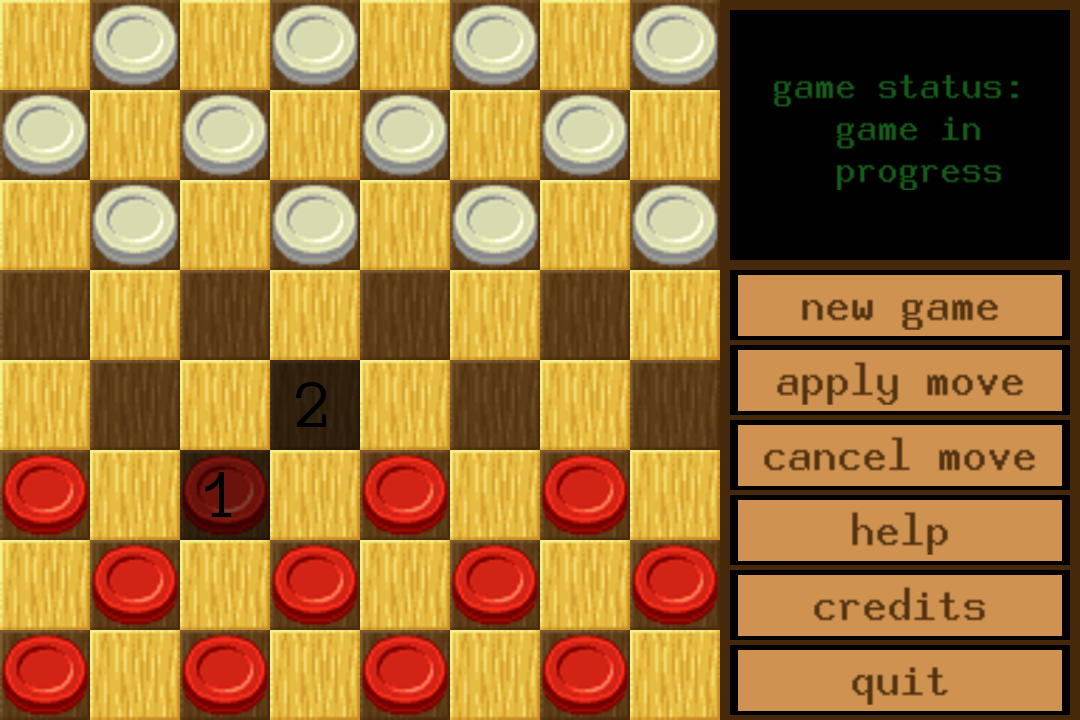
\includegraphics[width=8cm]{img/first_move.png}
	\caption{First move}
	\label{fig:first_move}
\end{figure}
\begin{figure}[hp]
	\centering
	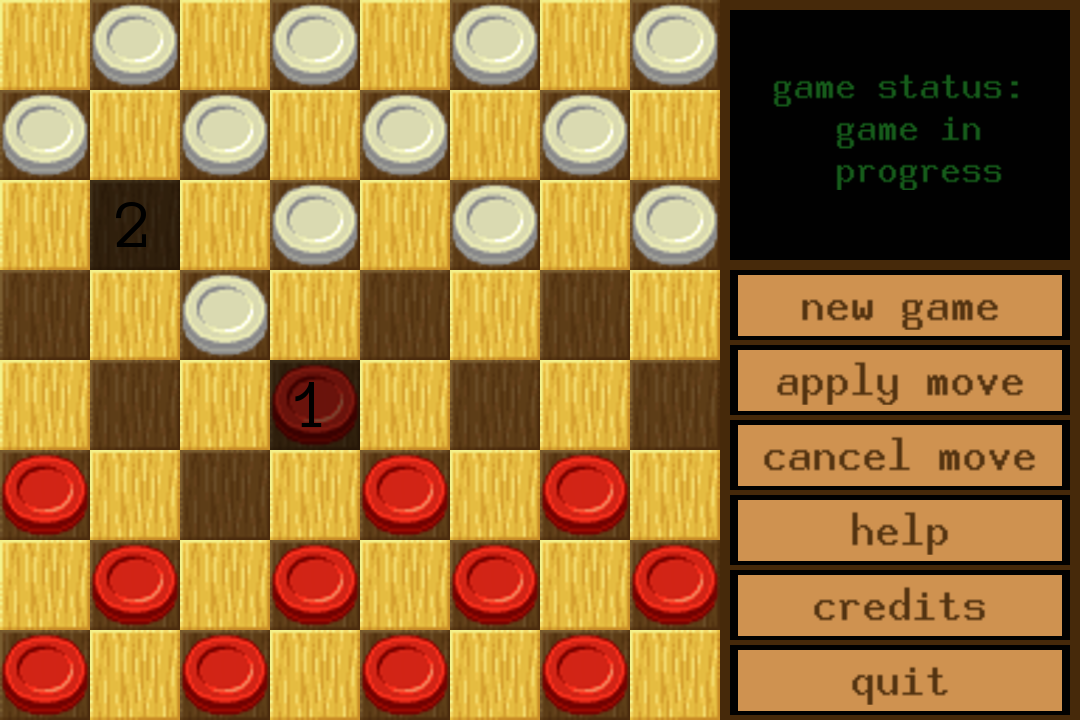
\includegraphics[width=8cm]{img/capture.png}
	\caption{Capture}
	\label{fig:capture}
\end{figure}
\begin{figure}[hp]
	\centering
	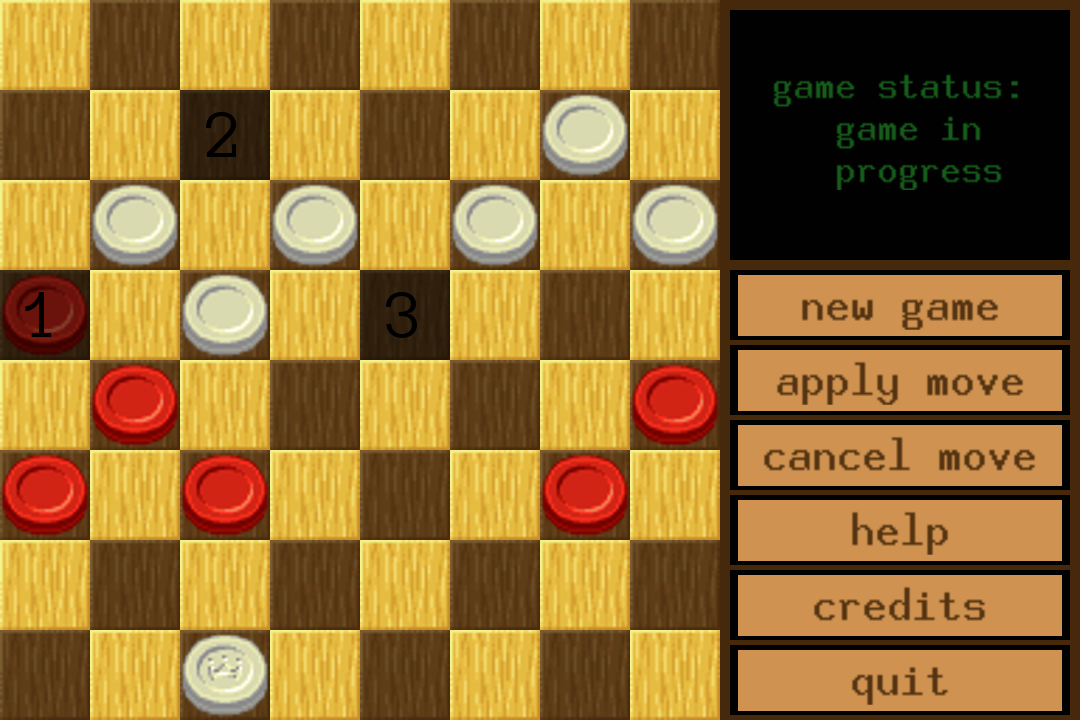
\includegraphics[width=8cm]{img/multiple_capture.png}
	\caption{Multiple capture}
	\label{fig:multiple_capture}
\end{figure}
\begin{figure}[hp]
	\centering
	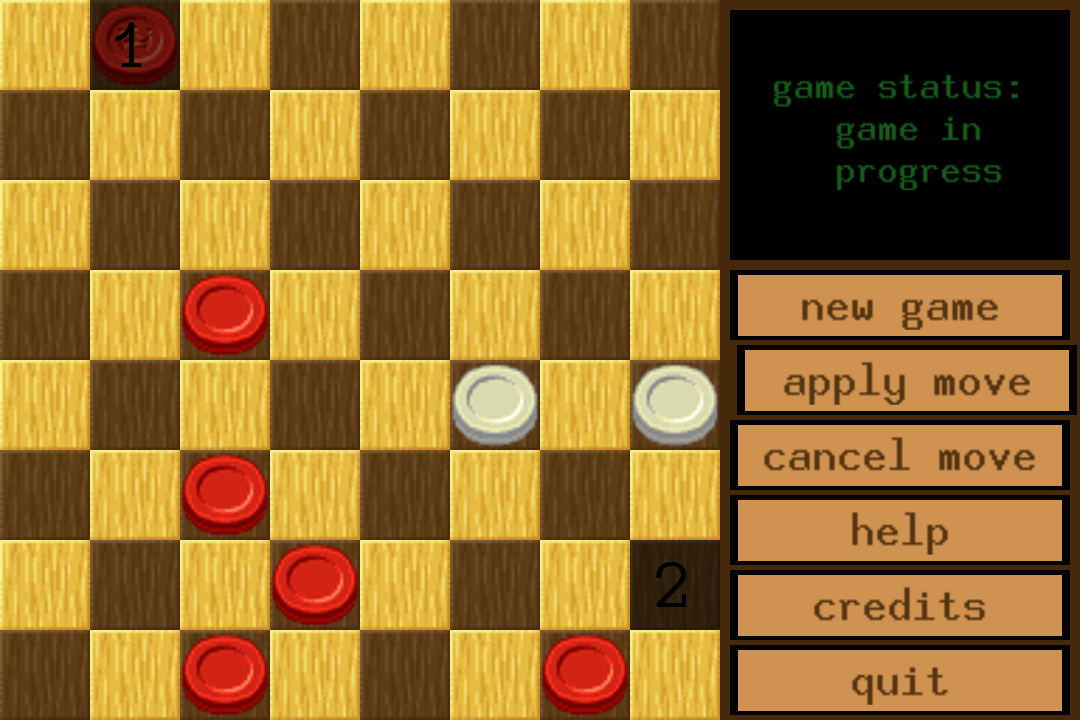
\includegraphics[width=8cm]{img/capture_with_king2.png}
	\caption{King capture}
	\label{fig:capture_with_king}
\end{figure}

\end{document}
